\documentclass[10pt,a4paper]{article}
\usepackage[utf8]{inputenc}
\usepackage[T1]{fontenc}
\usepackage[brazil]{babel}
\usepackage{lmodern}
\usepackage[margin=1.8cm]{geometry}
\usepackage{graphicx}
\usepackage{booktabs}
\usepackage{hyperref}
\usepackage{titlesec}
\titlespacing*{\section}{0pt}{1.0ex}{0.5ex}
\setlength{\parskip}{0.25ex}

\title{\vspace{-1.8cm}Nativo vs.\ contêiner: \texttt{osu\_bw} e \texttt{osu\_latency} no CENAPAD}
\author{Mateus Oliveira (m203656@dac.unicamp.edu.br), MO652}
\date{outubro de 2026}

\begin{document}
\maketitle
\vspace{-0.8cm}
\begin{center}
Repositório: \href{https://github.com/oliveiraMats2/compare_performance_CENAPAD}{github.com/oliveiraMats2/compare\_performance\_CENAPAD}
\end{center}

\section{Ambiente}
Dois nós CPU do CENAPAD (\texttt{adano07} e \texttt{adano21}, job \texttt{1027215.ada}, 06/10/2026), fila \texttt{paralela} com \texttt{select=2:\allowbreak ncpus=128:\allowbreak mpiprocs=1} e \texttt{place=scatter:exclhost}. Ambos têm HCA Mellanox ConnectX-6 (MT4123, \texttt{mlx5\_0}, firmware 20.43.3608), porta \emph{Active/LinkUp}, camada de enlace InfiniBand, taxa 100 Gb/s (HDR100).

\textbf{Nativo:} Spack v1.2.2 com GCC 8.5.0 (sistema, AlmaLinux 8): MPICH 5.0.1 (\texttt{ch4:ucx}), UCX 1.20.1 e OSU Micro-Benchmarks 7.5.2; a especificação concretizada está em \texttt{spack/spack.lock}.
\textbf{Contêiner:} receita HPCCM sobre \texttt{ubuntu:24.04}, GCC do \texttt{apt} do Ubuntu, com as mesmas versões de MPICH (5.0.1, \texttt{ch4:ucx}), UCX (1.20.1) e OSU (7.5.2), executada com Singularity.

\textbf{Pilha InfiniBand (desvio do enunciado).} Os nós \emph{não} têm Mellanox OFED: a pilha de espaço de usuário é o \texttt{rdma-core} 48.0 da própria distribuição (\texttt{rdma-core-48.0-1.el8}, \texttt{libibverbs-48.0-1.el8}). Por isso a receita compila o \texttt{rdma-core} 48.0 no contêiner (o Ubuntu 24.04 traz o 50.0) em vez do MOFED, igualando a versão do host (\texttt{libibverbs.so.1.14.48.0}). No host, o UCX do Spack foi ligado a um \texttt{rdma-core} 49.0 do próprio Spack (não há pacote 48.0). Isso é compatível porque o driver de kernel (\texttt{mlx5}) é o mesmo e a \texttt{libibverbs} mantém ABI estável entre essas versões.

\section{Procedimento}
Dois processos MPI, um por nó (\texttt{mpiexec -n 2 -ppn 1}), lançados pelo \texttt{mpiexec} do host em ambos os cenários; no contêiner ele executa \texttt{singularity exec} (modelo híbrido). Mensagens de 1 B a 4 MiB (\texttt{-m 1:4194304}), iterações padrão do OSU. Foram 3 repetições por teste e cenário, intercaladas no mesmo job (repetição $k$: bw nativo, bw contêiner, latência nativa, latência contêiner), nos mesmos nós. O uso de InfiniBand foi verificado com \texttt{UCX\_LOG\_LEVEL=info} e \texttt{UCX\_NET\_DEVICES=mlx5\_0:1}: nos dois cenários o UCX escolhe \texttt{inter-node cfg\#1 tag(rc\_mlx5/mlx5\_0:1) rma(rc\_mlx5/mlx5\_0:1)\ldots}, com 244 linhas de transporte \texttt{rc/dc/ud\_mlx5} e nenhuma de TCP (\texttt{logs/ib\_check.log}). Gráficos gerados por \texttt{analysis/plot.py}.

\section{Resultados}
\begin{figure}[h]
\centering
\begin{minipage}{0.49\textwidth}\centering
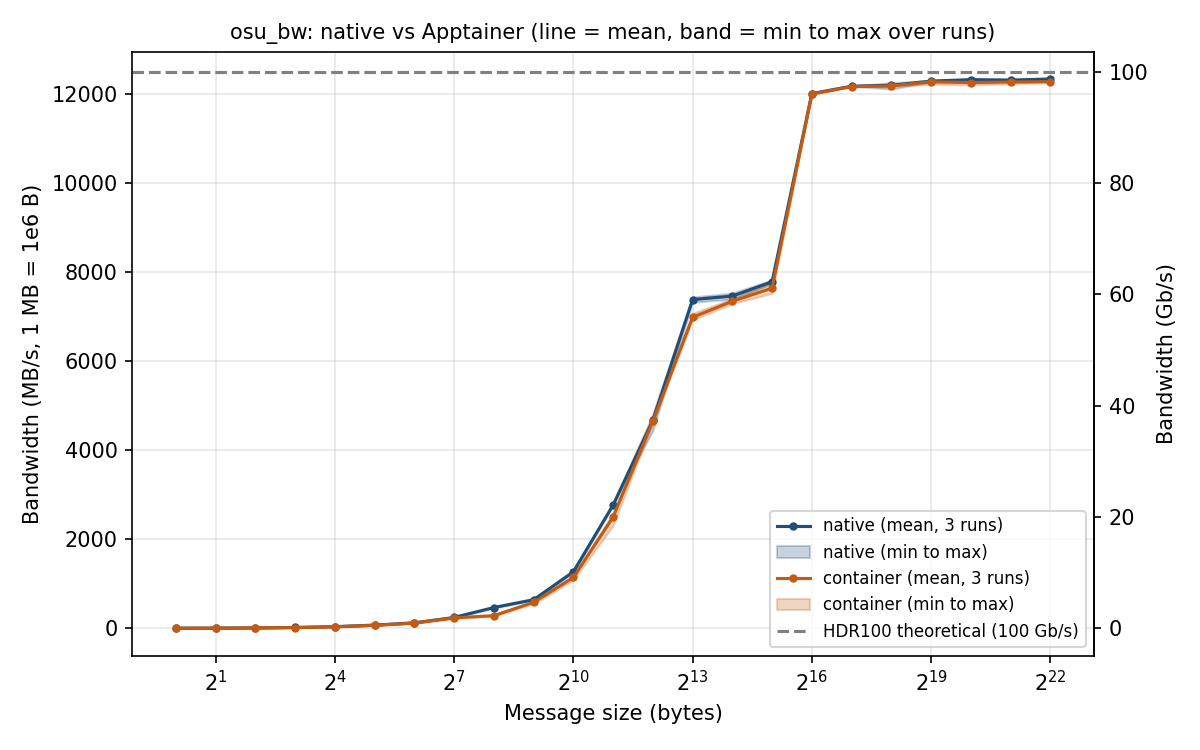
\includegraphics[width=\linewidth]{../figures/bandwidth.png}\\[-0.5ex]
{\small (a) Largura de banda (\texttt{osu\_bw})}
\end{minipage}\hfill
\begin{minipage}{0.49\textwidth}\centering
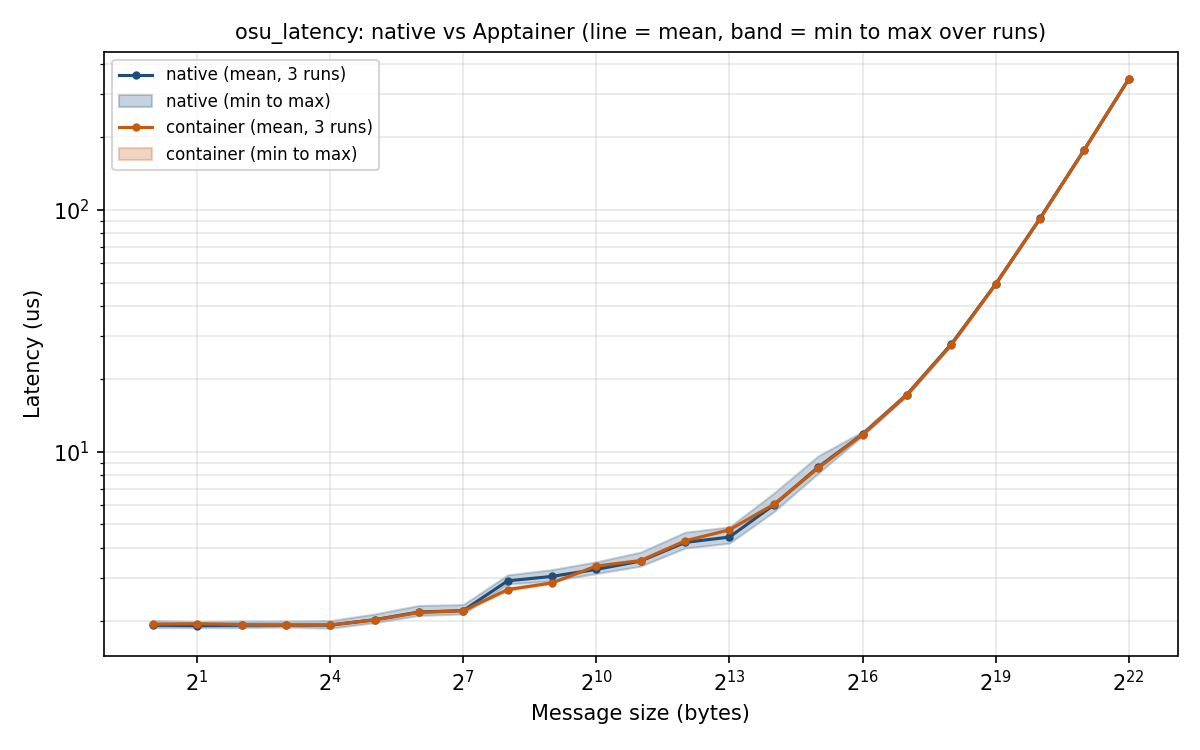
\includegraphics[width=\linewidth]{../figures/latency.png}\\[-0.5ex]
{\small (b) Latência (\texttt{osu\_latency})}
\end{minipage}
\vspace{-1ex}
\caption{Nativo vs.\ contêiner em função do tamanho da mensagem (eixo $x$ em escala $\log_2$). Linha: média de 3 execuções; faixa: mínimo a máximo.}
\end{figure}

\begin{table}[h]
\centering\small
\vspace{-2ex}
\begin{tabular}{lrrr}
\toprule
Métrica & Nativo & Contêiner & Diferença \\
\midrule
Banda média em 4 MiB (MB/s) & 12338,3 & 12277,0 & $-0{,}50$\,\% \\
Banda em 4 MiB (Gb/s, \% de 100 Gb/s) & 98,71 (98,7\,\%) & 98,22 (98,2\,\%) & \\
Banda média em 256 B (MB/s) & 457 a 472 & 267 a 294 & $-38{,}9$\,\% \\
Latência média em 1 B ($\mu$s) & 1,913 & 1,933 & $+1{,}05$\,\% \\
Latência média em 4 MiB ($\mu$s) & 347,11 & 347,18 & $\approx 0$ \\
CV máximo \texttt{osu\_bw} / \texttt{osu\_latency} & 4,30\,\% / 10,32\,\% & 11,11\,\% / 1,72\,\% & \\
\bottomrule
\end{tabular}
\caption{Valores principais (MB do OSU $=10^6$ B; em 256 B, faixa mínimo a máximo das 3 execuções e diferença das médias).}
\end{table}
\vspace{-3ex}

\section{Análise}
\textbf{Efeito do tamanho da mensagem.} Para mensagens pequenas domina o custo fixo por mensagem: a latência fica entre 1,91 e 1,94\,$\mu$s de 1 a 16 B e a banda é baixa. Para mensagens grandes domina a transferência: a latência praticamente dobra a cada duplicação do tamanho (347\,$\mu$s em 4 MiB) e a banda cresce até saturar o enlace.

\textbf{Banda máxima e percentual do teórico.} O OSU reporta MB/s com MB $=10^6$ B; como 1 MB/s $= 8$ Mb/s, Gb/s $=$ MB/s $\times 8 / 1000$. O pico médio nativo foi 12338,3 MB/s em 4 MiB $= 98{,}71$ Gb/s, ou 98,7\,\% dos 100 Gb/s; no contêiner, 12277,0 MB/s $= 98{,}22$ Gb/s (98,2\,\%).

\textbf{Estabilização.} Nos dois cenários a banda atinge pelo menos 95\,\% do pico a partir de 64 KiB e permanece nesse patamar. O salto de 32 KiB para 64 KiB (nativo 7783,9 para 12010,3 MB/s, $+54$\,\%; contêiner 7640,2 para 11998,9 MB/s, $+57$\,\%) coincide com a troca do protocolo \emph{eager} pelo \emph{rendezvous} (RDMA \emph{zero-copy}).

\textbf{Nativo vs.\ contêiner e consistência.} Onde a rede é o gargalo ($\geq 64$ KiB) o contêiner fica de $-0{,}06$\,\% a $-0{,}53$\,\% do nativo: custo irrelevante. As diferenças aparecem em mensagens pequenas e médias, onde pesa o custo de software por mensagem. Em 256 B o contêiner é 38,9\,\% mais lento, menor nas 3 execuções pareadas e com faixas disjuntas: diferença consistente e reprodutível; o mesmo vale, em menor grau, de 512 B a 2 KiB e em 8 KiB ($-5$ a $-10$\,\%). Já de 1 a 32 B a média cai 7 a 8\,\%, mas por uma única execução lenta do contêiner (a 2ª, cerca de 19\,\% abaixo das demais; a 1ª coincide com o nativo em 1\,\%), com faixas sobrepostas: não é robusta (o CV máximo do contêiner, 11,11\,\%, ocorre nessa faixa, em 8 B). Na latência os cenários ficam dentro de cerca de 2\,\% na maioria dos tamanhos; em 256 e 512 B o contêiner é mais rápido ($-8{,}0$ e $-6{,}0$\,\%) em parte porque a 1ª execução nativa foi sistematicamente mais lenta (5 a 14\,\% até 32 KiB, origem do CV de 10,32\,\%), e o $+7{,}2$\,\% em 8 KiB não é robusto (faixas sobrepostas, sinais mistos). Hipóteses, não verificadas, para as diferenças reais: compilações distintas de UCX/MPICH (Spack com otimizações vs.\ \texttt{configure} padrão no HPCCM), glibc/GCC diferentes e limiares de protocolo distintos.

\textbf{Distância ao limite teórico.} O pico ficou só 1,3\,\% abaixo dos 100 Gb/s. Os 100 Gb/s do HDR100 já são a taxa de dados após a codificação de linha, então ela não explica a diferença. Contribuem: cabeçalhos dos pacotes IB (LRH/BTH/ICRC) e créditos de controle de fluxo, sobrecarga de protocolo do MPI/UCX (\emph{handshake} do \emph{rendezvous}), registro de memória e o barramento PCIe. Mensagens pequenas ficam muito longe do limite por causa do custo fixo por mensagem (latência de cerca de 1,9\,$\mu$s).

\end{document}
